% Provenance (never printed): see sources/outline_sources.md (Year 2: oceanic islands; growth,
% flank collapse and erosion of volcanic islands; reefs and atolls; subsidence). Hawaiian
% stages, slides, subsidence and drowned reefs after Clague and Sherrod (2014, USGS PP 1801
% ch. 3) and Denlinger and Morgan (2014, ch. 4); the Nuuanu slide after the ODP Leg 200 report;
% the Enewetak holes after Ladd and Schlanger (1960, USGS PP 260-Y); Kure after the NOAA
% monument pages; the depth--age law from the Book 2 and Book 3 rows. Curves and the invented
% Petrel island from figdata/bachelor-2/islands.py; exercise and problem values in the Book 4
% scratch calculator calc/ch17.py.
\chapter{Îles océaniques}\label{ch:b2:oceanic-islands}

En 1952, sur deux îles de l'\omterm{def:b2:oceanic-islands:reefs}{atoll} d'Enewetak, dans le Pacifique occidental (alors orthographié Eniwetok), deux
sondages ont traversé la roche corallienne jusqu'à plus de \qty{1.2}{km}. Sur l'île Parry, le trépan a ramené
des débris de basalte frais à une profondeur de 4~158 pieds, soit \qty{1267}{m}, puis une carotte de basalte
à olivine. Au-dessus reposait un calcaire d'âge éocène, plein de coraux de récif d'une espèce qui ne croît
pas au-delà d'environ \qty{46}{m}. Un récif de corail avait jadis poussé sur les flancs d'un volcan proche
du niveau de la mer, et le volcan s'était enfoncé de plus d'un kilomètre pendant que le récif continuait
de croître par-dessus. Ce chapitre suit une \omterm{def:b2:oceanic-islands:stages}{île océanique} tout au long de sa vie~: comment elle croît, comment
ses flancs s'effondrent dans la mer, pourquoi elle s'enfonce, et comment un anneau de corail peut lui survivre.
% ledger: ls60:enewetak, ics4:eocene

\begin{recall}
\textbf{Du volume de première année}~: point chaud, panache mantellique, trace de point chaud et sa
progression en âge, chaîne Hawaï--Empereur et bombement hawaïen~; loi profondeur--âge du fond océanique~;
\omterm{def:b2:oceanic-islands:reefs}{récifs frangeants}, barrières et \omterm{def:b2:oceanic-islands:reefs}{atolls}, dans les formes que Darwin a décrites, et la règle «~garder
le niveau ou se noyer~»~; eustasie et niveau de la mer au dernier maximum glaciaire, environ \qty{120}{m}
plus bas qu'aujourd'hui. \textbf{Des volumes du secondaire}~: le volcan-bouclier~; la plate-forme
d'abrasion marine. \textbf{D'après le \cref{ch:b2:magmatic-series}}~: \omterm{def:b2:magmatic-series:series}{séries tholéiitique} et alcaline.
\end{recall}

\section{La croissance d'une île volcanique}\label{sec:b2:oceanic-islands:growth}

Les îles Hawaï forment l'extrémité la plus jeune de la chaîne que le volume de première année a
suivie à travers le nord du Pacifique. Les îles principales comptent 19 volcans-boucliers connus~: 15
s'élèvent au-dessus de la mer, 3 sont submergés, et un, né récemment, est encore sous l'eau. Au fur et
à mesure que la plaque Pacifique les emporte vers le nord-ouest, chacun naît au-dessus du point chaud,
grandit, meurt en s'éloignant et s'enfonce. Sa vie est assez régulière pour se découper en étapes.
% ledger: cs14:volcanoes

\begin{definition}[Île océanique~; étapes de la croissance]\label{def:b2:oceanic-islands:stages}
Une \emph{île océanique}\index{île océanique} est une île volcanique qui s'élève du fond de l'océan,
construite sur la lithosphère océanique. Une île d'une chaîne de point chaud traverse quatre stades
éruptifs~: un stade \emph{pré-bouclier} de petites éruptions de lave alcaline sur le fond marin~; le
\emph{stade bouclier}\index{stade bouclier}, où la lave tholéiitique édifie l'essentiel du volcan pendant
qu'il se trouve au-dessus du point chaud~; un stade \emph{post-bouclier} d'éruptions moins nombreuses
et plus alcalines, qui coiffent le bouclier~; et, après une pause, un stade \emph{de rajeunissement}
de rares petites éruptions alcalines. L'érosion et l'enfoncement prennent ensuite le relais.
\end{definition}
% ledger: usgs14:hawaii-stages, cs14:rejuvenated

Les stades suivent l'apport de chaleur. Loihi, le volcan le plus récent, se trouve à \qty{54}{km} au sud du
sommet du Kilauea~; son sommet est encore à \qty{975}{m} sous la mer, mais déjà à \qty{2.5}{km} au-dessus
du fond environnant, et ses plus anciennes laves sont alcalines. Au \omterm{def:b2:oceanic-islands:stages}{stade bouclier}, le volcan se trouve
au-dessus du point chaud et y est alimenté au débit le plus élevé. Chaque volcan hawaïen émet pendant ce stade
entre 80 et \qty{95}{\percent} de son volume final, surtout dans ses premiers \qty{1}{Ma} à \qty{2}{Ma}.
Vers la fin de ce stade, le débit d'éruption chute d'un facteur dix. Les réservoirs magmatiques
superficiels, à une profondeur de 1 à \qty{7}{km}, ne peuvent plus être entretenus, mais de plus petits,
situés à 20 à \qty{30}{km}, subsistent. La lave redevient alcaline, parce qu'un degré de fusion plus
faible la produit, comme l'a montré le \cref{ch:b2:magmatic-series}. Le stade de rajeunissement vient
après une pause de moins de 0.5 à \qty{2.0}{Ma}. Il peut compter un ou deux épisodes, ou durer très
longtemps~: à Niihau il a duré de 2.2 à \qty{0.4}{Ma}, et à Kauai il se poursuit depuis \qty{3.5}{Ma}.
% ledger: cs14:loihi, usgs14:hawaii-stages, cs14:rejuvenated

Les volumes sont énormes. Le volume du Mauna Loa est estimé à environ \qty{74000}{km^3}. Lorsque la limite
avec le Kilauea est redessinée, de sorte que le Kilauea ne garde qu'environ \qty{10000}{km^3}, la part du
Mauna Loa monte à \qty{95600}{km^3}. Le jeune Loihi en contient \qty{1700}{km^3}. L'ensemble de la chaîne,
depuis \qty{81}{Ma}, représente environ \qty{2e6}{km^3}~; un débit d'éruption intégré sur cette histoire, \qty{0.07}{km^3} par an, en donnerait près de trois fois plus. La
charge est assez lourde pour plier la plaque~: la croûte océanique sous les îles est enfoncée de jusqu'à
\qty{5}{km}, le long d'une dépression appelée fosse hawaïenne, et un léger bombement, l'arche hawaïenne,
se soulève à quelques centaines de kilomètres. Comment une plaque se plie sous une charge est traité dans
le volume de troisième année. Ici la fosse compte, car elle reçoit une grande partie des débris des îles.
% ledger: cs14:volumes, cs14:loihi, cs14:moat

\begin{omfigure}
\centering
\begin{tikzpicture}[x=0.95cm, y=0.95cm, font=\footnotesize]
% schematic, not to scale (vertical exaggeration about 10). Sea level y = 0; sea floor
% y = -1.6 - 0.0625 (16 - x), deepening with the age of the plate to the left.
\fill[omSea!45] (0,0) -- (16,0) -- (16,-1.6) -- (0,-2.6) -- cycle;
\fill[black!18] (0,-2.6) -- (16,-1.6) -- (16,-3.1) -- (0,-3.1) -- cycle;
\draw[black!60] (0,-2.6) -- (16,-1.6);
\draw[omSea!60!black] (0,0) -- (16,0);
\node[anchor=south, font=\scriptsize] at (8.7,0) {niveau de la mer};
% (a) shield stage over the hotspot
\fill[lith basalt, draw=black!70] (12.6,-1.8125) -- (13.9,0.75) -- (14.3,0.9) -- (14.7,0.75) -- (16,-1.6) -- cycle;
% (b) eroded island with a fringing reef (valleys notched in the summit)
\fill[lith basalt, draw=black!70] (9.2,-2.025) -- (10.1,0.15) -- (10.3,0.35) -- (10.45,0.2) -- (10.6,0.45) -- (10.8,0.25) -- (11.0,0.3) -- (11.2,0.1) -- (12.0,-1.85) -- cycle;
\fill[lith reef limestone, draw=black!70] (10.038,0) -- (9.976,-0.15) -- (9.80,0) -- cycle;
\fill[lith reef limestone, draw=black!70] (11.241,0) -- (11.303,-0.15) -- (11.46,0) -- cycle;
% (c) barrier reef around a smaller island, a lagoon between
\fill[lith basalt, draw=black!70] (5.8,-2.2375) -- (7.0,0.2) -- (8.2,-2.0875) -- cycle;
\fill[lith reef limestone, draw=black!70] (6.384,-1.05) -- (6.42,0) -- (6.60,0) -- (6.62,-0.45) -- (6.680,-0.45) -- cycle;
\fill[lith reef limestone, draw=black!70] (7.656,-1.05) -- (7.62,0) -- (7.44,0) -- (7.42,-0.45) -- (7.341,-0.45) -- cycle;
% (d) atoll: volcano bevelled and drowned, reef cap with a lagoon
\fill[lith basalt, draw=black!70] (2.7,-2.43125) -- (3.6,-0.55) -- (4.0,-0.55) -- (4.9,-2.29375) -- cycle;
\fill[lith reef limestone, draw=black!70] (3.4325,-0.9) -- (3.47,0) -- (4.14,0) -- (4.1806,-0.9) -- (4.0,-0.55) -- (3.6,-0.55) -- cycle;
\fill[omSea!45] (3.62,-0.15) rectangle (3.99,0);
% (e) guyot: flat top with a drowned reef cap, beyond the Darwin point
\fill[lith basalt, draw=black!70] (0.2,-2.5875) -- (0.9,-0.95) -- (1.7,-0.95) -- (2.4,-2.475) -- cycle;
\fill[lith reef limestone, draw=black!70] (0.9,-0.95) -- (0.96,-0.75) -- (1.64,-0.75) -- (1.7,-0.95) -- cycle;
% Darwin point
\draw[black!70, dashed] (2.55,0.55) -- (2.55,-2.5);
\node[anchor=south, font=\scriptsize] at (2.55,0.55) {point de Darwin};
% hotspot and plate motion
\draw[omThm, line width=1.4pt, -{Stealth[length=2.5mm]}] (14.3,-3.9) -- (14.3,-3.15);
\node[anchor=west, font=\scriptsize, text=omThm] at (14.4,-3.7) {point chaud};
\draw[black, line width=0.8pt, -{Stealth[length=2.5mm]}] (9.5,-2.85) -- (6.5,-2.85);
\node[anchor=west, font=\scriptsize] at (9.6,-2.85) {mouvement de la plaque};
\node[anchor=west, font=\scriptsize] at (0.1,-2.9) {lithosphère océanique};
% stage labels
\node[align=center, font=\scriptsize] at (14.3,1.45) {(a) stade bouclier};
\node[align=center, font=\scriptsize] at (10.6,1.3) {(b) île érodée,\\ récif frangeant};
\node[align=center, font=\scriptsize] at (7.0,1.45) {(c) récif-barrière};
\node[align=center, font=\scriptsize] at (3.8,1.45) {(d) atoll};
\node[align=center, font=\scriptsize] at (1.3,1.45) {(e) guyot};
\draw[black!60, -{Stealth[length=2mm]}] (13.6,-3.7) -- (0,-3.7);
\node[anchor=south, font=\scriptsize, fill=white, inner sep=1pt] at (7,-3.7) {volcans plus anciens, plaque plus ancienne et plus profonde};
\end{tikzpicture}
\par\smallskip{\small La vie d'une \omterm{def:b2:oceanic-islands:stages}{île océanique}, lue le long d'une chaîne de point chaud (schématique,
non à l'échelle, échelle verticale fortement exagérée). La plaque emporte chaque volcan loin du point
chaud (à droite) et le volcan s'enfonce avec elle, tandis que l'érosion l'use. (a)~Un volcan-bouclier
croît au-dessus du point chaud. (b)~Éteint et érodé, il est bordé de \omterm{def:b2:oceanic-islands:reefs}{récifs frangeants}. (c)~Enfoncé
davantage, il est entouré d'un \omterm{def:b2:oceanic-islands:reefs}{récif-barrière}, avec un lagon entre les deux. (d)~Son sommet a disparu
sous la mer, et une coiffe récifale entourant un lagon central, un \omterm{def:b2:oceanic-islands:reefs}{atoll}, croît par-dessus. (e)~Emporté
dans une eau trop froide pour que le récif suive, l'\omterm{def:b2:oceanic-islands:reefs}{atoll} se noie et s'enfonce en \omterm{def:b2:oceanic-islands:seamount}{guyot} à sommet plat.}
\end{omfigure}
% ledger: cs14:volcanoes, cs14:erase, cs14:darwin-point, pmnm:geology

\section{Effondrement de flanc}\label{sec:b2:oceanic-islands:collapse}

Un volcan de plusieurs kilomètres de haut, bâti de coulées de lave et de débris meubles, posé
sur des pentes qui descendent dans la fosse, n'est pas stable. En 1975, le séisme de Kalapana, de
magnitude 7.7, a déplacé d'un seul coup le flanc sud du Kilauea, jusqu'à \qty{10}{m} vers la mer, et
a provoqué un tsunami. En 1868, un autre mouvement de flanc a accompagné un séisme de magnitude 7.9
et un tsunami qui a tué 46 personnes. Les profils sismiques sous ces flancs montrent un réflecteur
profond. Il est interprété comme un \omterm{def:b2:alpine-orogen:decollement}{décollement} le long du sommet de l'ancienne croûte océanique,
sur lequel glisse tout le flanc. Le plus souvent, le flanc se déforme lentement~; parfois il cède.
% ledger: dm14:flank

\begin{definition}[Effondrement de flanc~; avalanche de débris~; glissement rotationnel]\label{def:b2:oceanic-islands:collapse}
Un \emph{effondrement de flanc}\index{effondrement de flanc} est la rupture d'une grande partie du flanc
d'un volcan, qui glisse sous son propre poids. Lorsque la masse en mouvement se fragmente et s'écoule
vite, sous forme de blocs et de débris capables de voyager loin au-delà du pied du volcan, c'est une
\emph{avalanche de débris}\index{avalanche de débris}. Lorsqu'elle se déplace lentement, en gros blocs qui tournent sur
des failles enracinées dans un \omterm{def:b2:alpine-orogen:decollement}{décollement} profond et restent près du volcan, c'est un \emph{glissement rotationnel}.
\end{definition}

Les preuves sont sous la mer. À la fin des années 1980, la cartographie au sonar à balayage latéral
des eaux autour des îles Hawaï a révélé des débris répandus sur le fond profond, à plusieurs centaines
de kilomètres des îles, et des glissements faits de grands blocs segmentés. Dix-sept grands glissements
ont été identifiés autour des îles principales, formés au cours des \qty{5}{Ma} passés. Soixante-dix
sont aujourd'hui connus le long de la dorsale hawaïenne, entre l'île d'Hawaï et Midway, formés
en \qty{30}{Ma}. Cela fait au moins un glissement tous les \qty{300}{ka} autour des îles principales.
Ces comptes sont des minima, car un volcan plus jeune peut enfouir la cicatrice et les débris
d'un plus ancien~: la \omterm{def:b2:eruptive-styles:caldera}{caldeira} sommitale et une zone de rift de Niihau manquent, et aucun dépôt n'a été
trouvé pour eux. Les grands glissements semblent les plus probables pendant que le volcan croît le plus
vite, du stade pré-bouclier tardif au stade post-bouclier précoce, mais ils se poursuivent bien après.
% ledger: cs14:slides, dm14:flank

Le plus grand est le glissement de Nuuanu, qui a arraché le flanc nord-est du volcan
Koolau, à Oahu. C'est une \omterm{def:b2:oceanic-islands:collapse}{avalanche de débris} étalée sur \qty{23000}{km^2}, qui s'étend à
plus de \qty{200}{km} de l'île. Parmi ses blocs figure le \omterm{def:b2:oceanic-islands:seamount}{mont sous-marin} Tuscaloosa, long
d'environ \qty{30}{km}, large de \qty{17}{km} et haut d'au moins \qty{2}{km}. L'avalanche
a traversé la fosse profonde et a grimpé à plus de \qty{100}{km} sur la pente de l'arche
hawaïenne. Son âge est estimé à 2.1 à \qty{1.8}{Ma}, vers la fin de la vie du Koolau ou
après celle-ci, dont les laves de surface ont 1.8 à \qty{2.6}{Ma}. Combien d'effondrements
l'ont formée, et quelle est son épaisseur loin de l'île, restent des questions ouvertes.
% ledger: odp200:nuuanu

\begin{omfigure}
\centering
\begin{tikzpicture}[x=0.95cm, y=0.95cm, font=\footnotesize]
% schematic section from the summit of an island (left) across the moat to the arch (right);
% not to scale. Sea level y = 0; top of the old oceanic crust, bent down under the island.
\fill[omSea!45] (0,0) -- (15,0) -- (15,-2.2) -- (13.5,-2.12) -- (11,-2.05) -- (8.5,-2.35) -- (6.5,-2.75) -- (5.6,-2.82) -- (4.0,-1.4) -- (2.5,0) -- cycle;
\fill[black!18] (0,-3.05) -- (5.6,-2.82) -- (6.5,-2.75) -- (8.5,-2.35) -- (11,-2.05) -- (13.5,-2.12) -- (15,-2.2) -- (15,-3.6) -- (0,-3.6) -- cycle;
\draw[black!70] (0,-3.05) -- (5.6,-2.82) -- (6.5,-2.75) -- (8.5,-2.35) -- (11,-2.05) -- (13.5,-2.12) -- (15,-2.2);
\draw[omSea!60!black] (0,0) -- (15,0);
\node[anchor=south east, font=\scriptsize] at (15,0) {niveau de la mer};
% the volcano: present flank (after collapse) and the lost flank (dashed)
\fill[lith basalt, draw=black!70] (0,1.15) -- (0.8,1.05) -- (1.25,0.95) -- (1.45,0.45) -- (1.75,0.1) -- (2.6,-0.75) -- (3.6,-1.6) -- (4.6,-2.4) -- (5.6,-2.82) -- (0,-3.05) -- cycle;
\draw[black!70, dashed] (1.25,0.95) -- (2.5,0) -- (4.0,-1.4) -- (5.6,-2.82);
\node[font=\scriptsize, align=center, fill=white, inner sep=1pt] at (0.8,-1.6) {volcan};
\node[font=\scriptsize, anchor=south west, align=left] at (2.0,0.25) {cicatrice du\\ flanc disparu};
% slump: blocks rotated on listric faults rooted in the decollement
\draw[black, line width=0.7pt] (1.45,0.45) .. controls (1.7,-1.4) and (2.4,-2.6) .. (3.6,-2.95);
\draw[black, line width=0.7pt] (2.6,-0.75) .. controls (2.8,-1.8) and (3.3,-2.6) .. (4.4,-2.9);
\draw[omThm, line width=1.1pt] (0.6,-3.03) -- (5.6,-2.82);
\node[anchor=north, font=\scriptsize, text=omThm] at (2.9,-3.05) {décollement};
% debris avalanche: hummocky sheet across the moat and up the arch, with blocks
\fill[lith conglomerate, draw=black!70] (4.6,-2.4) -- (5.6,-2.62) -- (6.5,-2.6) -- (8.5,-2.22) -- (11,-1.95) -- (12.6,-2.03) -- (11,-2.05) -- (8.5,-2.35) -- (6.5,-2.75) -- (5.6,-2.82) -- cycle;
\fill[lith basalt, draw=black!70] (7.0,-2.62) -- (7.25,-2.25) -- (7.95,-2.22) -- (8.1,-2.43) -- cycle;
\fill[lith basalt, draw=black!70] (9.3,-2.2) -- (9.45,-2.02) -- (9.75,-2.0) -- (9.85,-2.17) -- cycle;
\fill[lith basalt, draw=black!70] (10.6,-2.05) -- (10.7,-1.93) -- (10.9,-1.92) -- (10.95,-2.03) -- cycle;
\draw[black!70] (7.6,-2.2) -- (7.4,-1.3) node[anchor=south, font=\scriptsize, align=center] {bloc de plusieurs\\ km de large};
\node[anchor=south, font=\scriptsize, align=center] at (10.3,-1.3) {avalanche de débris};
\draw[black!70] (10.3,-1.3) -- (10.0,-1.98);
\node[font=\scriptsize] at (6.6,-3.2) {fosse};
\node[font=\scriptsize] at (11.6,-2.6) {arche};
\node[anchor=west, font=\scriptsize] at (12.6,-3.3) {croûte océanique};
\draw[black!70] (2.55,-1.55) -- (3.35,-0.6) node[anchor=west, font=\scriptsize, inner sep=1pt] {glissement rotationnel};
\draw[black!60, {Stealth[length=2mm]}-{Stealth[length=2mm]}] (5.6,-3.95) -- (12.6,-3.95);
\node[anchor=north, font=\scriptsize] at (9.1,-3.95) {jusqu'à environ \qty{200}{km}};
\end{tikzpicture}
\par\smallskip{\small \omterm{def:b2:oceanic-islands:collapse}{Effondrement de flanc} d'une \omterm{def:b2:oceanic-islands:stages}{île océanique} (schématique, non à l'échelle). Près du
volcan, un glissement rotationnel se déplace lentement en blocs qui tournent sur des failles enracinées
dans un \omterm{def:b2:alpine-orogen:decollement}{décollement}, au sommet de l'ancienne croûte océanique. Une \omterm{def:b2:oceanic-islands:collapse}{avalanche de débris} se détache du flanc,
laisse une cicatrice et s'étale en une nappe de débris portant des blocs larges de plusieurs kilomètres.
L'avalanche de Nuuanu a franchi la fosse et grimpé sur l'arche, à plus de \qty{200}{km} d'Oahu.}
\end{omfigure}
% ledger: dm14:flank, odp200:nuuanu, cs14:moat

Un glissement qui tombe dans la mer repousse l'eau. À Lanai et à Molokai, des brèches chaotiques de corail et de
lave s'élèvent jusqu'à \qty{155}{m} au-dessus du niveau de la mer et ont été interprétées comme les dépôts de vagues
géantes provoquées par des effondrements. Cette interprétation est contestée. Certains auteurs expliquent ces dépôts
par un soulèvement des îles, bien que les récifs noyés au sud de Lanai ne montrent aucun signe d'un tel soulèvement.
Environ un tiers des grands glissements hawaïens étaient des \omterm{def:b2:oceanic-islands:collapse}{avalanches de débris} capables de soulever d'énormes
vagues. Comment évaluer un tel aléa géologique, rare mais très grave, est traité au \cref{ch:b2:geological-hazards}.
% ledger: cs14:megatsunami

\section{Pourquoi les îles océaniques s'enfoncent}\label{sec:b2:oceanic-islands:subsidence}

Deux processus font s'enfoncer une \omterm{def:b2:oceanic-islands:stages}{île océanique}, et ils se recouvrent en partie. Le premier est
la charge~: à mesure que le volcan croît, son poids enfonce la plaque. Cette phase rapide dure
peut-être un million d'années et noie les rivages et les récifs de plus d'un kilomètre. Au large
de la côte nord-ouest de l'île d'Hawaï, des récifs noyés datés donnent une vitesse d'enfoncement
de \qty{2.6}{m} par millier d'années. Un petit volcan peut être entièrement noyé pendant cette
phase~: Mahukona, à côté de l'île d'Hawaï, a été brièvement une île, et son sommet se trouve
aujourd'hui à environ \qty{1100}{m} sous l'eau. Le second processus est le refroidissement de la
plaque, qui se poursuit pendant cent millions d'années, et dont cette section donne les chiffres.
% ledger: cs14:subsidence, cs14:mahukona

Le volume de première année a mesuré comment le fond océanique s'approfondit
avec son âge $t$ (en \unit{Ma}). Sous la forme utilisée dans ce chapitre~:
\[
d(t) = \qty{2500}{m} + C\sqrt{t}, \qquad C = \qty{350}{m.Ma^{-1/2}}, \qquad 0 \le t \le 70,
\]
et, pour des plaques plus âgées qu'environ \qty{20}{Ma},
\[
d(t) = \qty{6400}{m} - \qty{3200}{m}\; e^{-t/62.8}.
\]
Les deux formes concordent à environ \qty{20}{m} près
entre 20 et \qty{50}{Ma}, et se croisent à \qty{26}{Ma}.
% ledger: ps77:depth-age (Book 2), parsons:plate-model (Book 3)
% values (islands.py): t_switch 26.27, d_switch 4293.8; root - exp: 20 Myr -7.6, 50 Myr +18.3

\begin{proposition}[Enfoncement thermique d'une île]\label{prop:b2:oceanic-islands:sinking}
Une île bâtie sur une plaque d'âge $t_1$, portée par la plaque, qui la charge d'un poids
qui ne change plus, et sans modifier le refroidissement de la plaque sous elle, s'enfonce de
\[
S = d(t_2) - d(t_1)
\]
à l'instant où la plaque a atteint l'âge $t_2$, au rythme $\dot S = d'(t)$. Avec la loi en racine,
\[
S = C\left(\sqrt{t_2} - \sqrt{t_1}\right), \qquad \dot S = \frac{C}{2\sqrt t},
\]
et, avec la loi exponentielle, $\dot S = (\qty{3200}{m}/\qty{62.8}{Ma})\,e^{-t/62.8}$. Sur
un intervalle donné, une plaque jeune entraîne ses îles plus bas qu'une plaque ancienne.
\end{proposition}

\begin{proof}
Comparer deux colonnes de la plaque, de même âge, l'une sous l'île et l'autre sous l'océan ouvert, loin de là. Les deux se
refroidissent de la même façon, puisque l'île laisse inchangé le refroidissement de la plaque. Elles se contractent donc de
la même quantité, et le sommet de chacune descend de la même hauteur. Le poids propre de l'île est déjà compensé et ne change
plus, de sorte qu'il n'ajoute rien. La colonne océanique s'enfonce de $d(t_2) - d(t_1)$, et l'île aussi. Dériver donne le taux.
Pour la dernière affirmation, sur un intervalle fixe $\Delta$, $C(\sqrt{t_1 + \Delta} -
\sqrt{t_1})$ décroît quand $t_1$ croît, car sa dérivée, $\frac C2\bigl(1/\sqrt{t_1 + \Delta}
- 1/\sqrt{t_1}\bigr)$, est négative.
\end{proof}

La proposition laisse volontairement de côté deux éléments. Le bombement du point chaud soulève la plaque
lorsqu'elle passe, puis la laisse redescendre en s'éloignant, ce qui s'ajoute à l'enfoncement des îles
les plus jeunes (le volume de première année a mesuré ce bombement). Et une charge change pendant que le
volcan croît, ce qui est la phase rapide ci-dessus. Une fois ces deux phases achevées, l'île suit le fond.

Les taux sont faibles. Sur une plaque âgée de \qty{4}{Ma}, la loi en racine donne \qty{87.5}{m} par
million d'années, soit moins d'un dixième de millimètre par an. Sur une plaque de \qty{100}{Ma}, la
loi exponentielle donne \qty{10.4}{m} par million d'années, soit \qty{0.01}{m} par millier d'années.
C'est le taux mesuré le long d'une bonne partie de la dorsale hawaïenne et des \omterm{def:b2:oceanic-islands:seamount}{monts sous-marins}
Empereur. La phase de charge, à \qty{2.6}{m} par millier d'années, est environ 250 fois plus rapide.
% ledger: cs14:subsidence; values (islands.py): rate_100 10.37, age_rate10 102.3

\begin{omfigure}
\centering
% figdata/bachelor-2/islands.py part sink
\begin{tikzpicture}
\begin{axis}[width=0.8\linewidth, height=6.2cm, y dir=reverse, xmin=0, xmax=100, ymin=0,
  ymax=3000, xlabel={temps depuis la construction de l'île (\unit{Ma})},
  ylabel={enfoncement thermique (\unit{m})}, tick label style={font=\scriptsize},
  label style={font=\small}, xtick pos=bottom, ytick pos=left]
\addplot[omThm, line width=1pt] table[x=dt_Myr, y=t2] {figdata/out/bachelor-2-islands-sink.dat};
\addplot[orange!80!black, line width=1pt] table[x=dt_Myr, y=t10] {figdata/out/bachelor-2-islands-sink.dat};
\addplot[blue!70!black, line width=1pt] table[x=dt_Myr, y=t30] {figdata/out/bachelor-2-islands-sink.dat};
\addplot[black!45, line width=1pt] table[x=dt_Myr, y=t60] {figdata/out/bachelor-2-islands-sink.dat};
\node[font=\scriptsize, anchor=south east, inner sep=1pt] at (axis cs:99,2470) {plaque de \qty{2}{Ma}};
\node[font=\scriptsize, anchor=south east, inner sep=1pt] at (axis cs:99,2140) {\qty{10}{Ma}};
\node[font=\scriptsize, anchor=south east, inner sep=1pt] at (axis cs:99,1380) {\qty{30}{Ma}};
\node[font=\scriptsize, anchor=south east, inner sep=1pt] at (axis cs:99,710) {\qty{60}{Ma}};
\draw[black!50, dashed] (axis cs:0,1267) -- (axis cs:58,1267);
\node[font=\scriptsize, anchor=north west, inner sep=1pt] at (axis cs:1,1300) {Enewetak, \qty{1267}{m}};
\end{axis}
\end{tikzpicture}
\par\smallskip{\small Enfoncement thermique d'une île portée par sa plaque, d'après la loi
profondeur--âge, pour des îles bâties sur des plaques âgées de 2, 10, 30 et \qty{60}{Ma} (la loi en racine
jusqu'à un âge de plaque de \qty{26}{Ma}, la loi exponentielle au-delà, là où les deux se rejoignent).
Plus la plaque est jeune, plus l'île s'enfonce vite et loin. La ligne en tirets marque la profondeur
du basalte sous Enewetak, soit l'épaisseur de roche récifale que l'enfoncement doit pouvoir accueillir.}
\end{omfigure}
% ledger: ps77:depth-age (Book 2), parsons:plate-model (Book 3), ls60:enewetak

\section{Récifs, atolls et guyots}\label{sec:b2:oceanic-islands:reefs}

Le volume de première année a décrit les trois formes de récifs telles que Darwin les expliquait,
d'un \omterm{def:b2:oceanic-islands:reefs}{récif frangeant} d'île jusqu'à un anneau de corail autour d'un lagon, et s'est terminé
sur une question~: pourquoi les îles s'enfoncent-elles, et jusqu'où~? La section précédente y
a répondu. Les formes peuvent maintenant être définies par l'état de l'île qui se trouve dessous.

\begin{definition}[Récif frangeant~; récif-barrière~; atoll]\label{def:b2:oceanic-islands:reefs}
Un \emph{récif frangeant}\index{récif frangeant} est un récif attaché au rivage d'une île, sans lagon, ou seulement
séparé de celle-ci par un chenal étroit et peu profond. Un \emph{récif-barrière}\index{récif-barrière} est
un récif séparé du rivage par un lagon, sur les flancs d'une île qui s'est enfoncée pendant que le récif croissait
vers le haut. Un \emph{atoll}\index{atoll} est un anneau de récif, avec de petites îles de débris récifaux, autour
d'un lagon sans roche volcanique au-dessus du niveau de la mer~: son volcan se trouve entièrement sous le récif.
\end{definition}

\begin{definition}[Mont sous-marin~; guyot]\label{def:b2:oceanic-islands:seamount}
Un \emph{mont sous-marin}\index{mont sous-marin} est un volcan du fond océanique dont le sommet
se trouve sous le niveau de la mer, soit parce qu'il n'a jamais atteint la surface, soit parce
qu'il s'est enfoncé. Un \emph{guyot}\index{guyot} est un mont sous-marin à sommet plat, raboté
par les vagues ou coiffé d'un récif lorsqu'il se trouvait au niveau de la mer, puis noyé.
\end{definition}

Si un récif maintient son sommet au niveau de la mer pendant que le volcan s'enfonce sous lui, la roche
récifale s'accumule aussi vite que l'île descend. L'épaisseur de la coiffe enregistre alors l'enfoncement.

\begin{proposition}[Épaisseur d'une coiffe récifale]\label{prop:b2:oceanic-islands:cap}
Soit $t_1$ l'âge de la plaque lorsque la dernière roche volcanique d'une île passe sous le niveau de
la mer, et soit un récif qui maintient son sommet au niveau de la mer à partir de ce moment, jusqu'à
ce que la plaque ait l'âge $t_2$. Si le niveau de la mer s'est élevé de $\Delta\eta$ entre les
deux instants (par rapport au centre de la Terre), alors la coiffe récifale au-dessus du volcan est
\[
H = d(t_2) - d(t_1) + \Delta\eta = C\left(\sqrt{t_2} - \sqrt{t_1}\right) + \Delta\eta
\]
épaisse, la seconde forme utilisant la loi en racine. Elle ne dépend pas du taux auquel le récif
peut croître, pourvu que ce taux ne soit jamais inférieur à la remontée relative du niveau de la mer.
\end{proposition}

\begin{proof}
À $t_1$, le sommet du volcan est au niveau de la mer~; à $t_2$, il se trouve $S = d(t_2) - d(t_1)$ plus
bas, selon la \cref{prop:b2:oceanic-islands:sinking}, tandis que la surface de la mer s'est élevée de
$\Delta\eta$. Le sommet du récif est à la surface de la mer aux deux instants, et sa base est le sommet du
volcan. L'épaisseur est donc la distance qui les sépare, soit $S + \Delta\eta$. Un récif qui suit la montée
reste à la surface, si bien qu'un récif plus rapide ne construit pas une coiffe plus épaisse~; un récif qui
ne peut suivre prend du retard et se noie, conformément à la règle rappelée du volume de première année.
\end{proof}

Enewetak le confirme. Avec la loi en racine, une coiffe de \qty{1267}{m} exige $\sqrt{t_2} - \sqrt{t_1} =
1267/350 = 3.62$~: par exemple un volcan arasé au niveau de la mer sur une plaque âgée de \qty{10}{Ma} et entraîné jusqu'à ce que la plaque ait \qty{46}{Ma}.
Cela fait \qty{36}{Ma}, l'ordre de grandeur du temps qui sépare la base éocène du
calcaire d'aujourd'hui. Les forages ont aussi montré ce que la proposition laisse de
côté. Les zones lessivées, où l'aragonite des coraux a été dissoute ou recristallisée,
enregistrent des époques où le sommet de l'\omterm{def:b2:oceanic-islands:reefs}{atoll} se trouvait au-dessus de la mer et où la
pluie tombait dessus. Le niveau de la mer monte et descend avec les âges glaciaires, et la
coiffe a été exposée puis noyée de nouveau de nombreuses fois au cours de son enfoncement.
% ledger: ls60:enewetak, ics4:eocene; calc/ch17.py: (3.162 + 3.620)^2 = 46.0

\begin{history}[Forages à travers les atolls, 1896--1952]
La théorie de Darwin faisait une prédiction qui ne pouvait être vérifiée qu'à l'aide d'un forage~: sous un
\omterm{def:b2:oceanic-islands:reefs}{atoll}, il devait exister une épaisse masse de roche récifale d'eau peu profonde, reposant sur de la roche
volcanique. Le premier sondage profond sur un \omterm{def:b2:oceanic-islands:reefs}{atoll} du Pacifique fut foré à Funafuti de 1896 à 1898 et
s'arrêta à 1~114 pieds, soit \qty{340}{m}, sans atteindre le volcan. Un forage à Kita-daito-jima, au sud du
Japon et à l'est d'Okinawa, atteignit 1~416 pieds en 1936, et un autre à Bikini 2~556 pieds en 1947~; ni l'un
ni l'autre n'atteignit le volcan. Les forages d'Enewetak, en 1951 et 1952, furent les premiers à atteindre le
socle d'un \omterm{def:b2:oceanic-islands:reefs}{atoll}. Sur l'île Elugelab, le socle dur fut rencontré à 4~610 pieds~; sur l'île Parry, le basalte
à 4~158 pieds, soit 450 pieds plus haut, à \num{22}~milles de là. Les foreurs avaient trouvé un volcan
basaltique qui s'élève de deux milles au-dessus du fond océanique, coiffé de calcaire récifal depuis l'éocène.
L'île Elugelab fut détruite lors d'un essai d'un dispositif thermonucléaire peu après la fin des forages.
\end{history}
% ledger: ls60:holes, ls60:enewetak

\begin{omfigure}
\centering
% figdata/bachelor-2/islands.py part holes
\begin{tikzpicture}
\begin{axis}[width=0.8\linewidth, height=6.0cm, ybar, bar width=16pt, y dir=reverse, ymin=0,
  ymax=1500, enlarge x limits=0.1, symbolic x coords={Funafuti,Kita-daito-jima,Bikini,Eniwetok-K-1B,Eniwetok-F-1,Eniwetok-E-1},
  xtick=data, xticklabels={{Funafuti\\1898},{Kita-daito-jima\\1936},{Bikini\\1947},{Enewetak\\K-1B, 1951},{Enewetak\\F-1, 1952},{Enewetak\\E-1, 1952}},
  xticklabel style={align=center, font=\scriptsize}, ylabel={profondeur (\unit{m})},
  tick label style={font=\scriptsize}, label style={font=\small}, xtick pos=bottom, ytick pos=left]
\addplot[fill=omLithLime, draw=black!70] table[x=name, y=td_m] {figdata/out/bachelor-2-islands-holes.dat};
\addplot[only marks, mark=-, mark size=9pt, line width=2.2pt, black, unbounded coords=discard, xshift=0pt]
  table[x=name, y=basalt_m] {figdata/out/bachelor-2-islands-holes.dat};
\end{axis}
\end{tikzpicture}
\par\smallskip{\small Les forages profonds réalisés sur les \omterm{def:b2:oceanic-islands:reefs}{atolls} du Pacifique, avec
l'année de leur achèvement~: leur profondeur totale (barres) et, à Enewetak, la profondeur
du socle basaltique (repères noirs) (\qty{1405}{m} sous Elugelab, F-1~; \qty{1267}{m}
sous l'île Parry, E-1). Profondeurs converties à partir des pieds du rapport de forage.}
\end{omfigure}
% ledger: ls60:holes, ls60:enewetak; values (islands.py): td and basalt in m

\begin{inthefield}[Forer un atoll]
À Enewetak, les géologues ont placé les sondages profonds près du rivage du lagon, où ils s'attendaient à moins de
cavités qu'au bord extérieur du récif. La plus grande partie du forage a été menée en ligne droite, la roche étant
broyée en débris que le fluide de forage remontait. Les débris remontaient en retard, si bien que l'équipe a estimé
ce décalage pour savoir de quelle profondeur provenait chaque échantillon. À des profondeurs choisies, un tube
carottier prélevait un cylindre de roche massive. Une fois le forage achevé, les trous ont servi d'instruments.
Dans l'un d'eux, tubé et cimenté jusqu'à \qty{600}{m}, le niveau de l'eau montait et descendait encore
avec la marée océanique, en phase et de la même amplitude~: le calcaire de la coiffe est poreux et plein de cavités
dans toute son épaisseur. D'autres ont mesuré la température dans les trous pendant leur retour à l'équilibre.
\end{inthefield}
% ledger: ls60:methods, ls60:casing (F-1 cased to 1,973 ft = 601 m)

Un récif n'est pas condamné à se noyer parce que son île s'enfonce. Les coraux et les algues corallines
s'accumulent à raison de quelques millimètres par an~: dans une étude récente, des récifs dominés par des
coraux branchus ont crû de \qty{4.2}{mm} par an. La plaque qui se refroidit retire au plus un dixième de
millimètre par an. L'enfoncement thermique seul ne dépassera jamais un récif en bonne santé. Les récifs
se noient lorsque autre chose change~: la plaque les emporte dans une eau trop froide pour une croissance
rapide~; le niveau de la mer monte plus vite qu'ils ne peuvent le suivre~; ou les deux se produisent à la fois.
% ledger: perry:chagos (Book 3), cs14:darwin-point

\begin{omfigure}
\centering
% figdata/bachelor-2/islands.py part rates; horizontal lines from the ledger rows
\begin{tikzpicture}
\begin{semilogyaxis}[width=0.8\linewidth, height=6.4cm, xmin=0, xmax=150, ymin=0.005, ymax=100,
  xlabel={âge de la plaque (\unit{Ma})}, ylabel={vitesse (\unit{mm.an^{-1}})},
  tick label style={font=\scriptsize}, label style={font=\small}, xtick pos=bottom, ytick pos=left]
\addplot[omThm, line width=1.1pt] table[x=t_Myr, y=thermal_mm_yr] {figdata/out/bachelor-2-islands-rates.dat};
\draw[omThm, densely dotted, line width=0.9pt] (axis cs:75,0.01) -- (axis cs:150,0.01);
\node[font=\scriptsize, anchor=south west, inner sep=1pt, text=omThm] at (axis cs:22,0.042) {enfoncement thermique de la plaque};
\node[font=\scriptsize, anchor=south west, inner sep=1pt, text=omThm] at (axis cs:96,0.0108) {mesuré, dorsale hawaïenne};
\draw[black!70, line width=0.9pt] (axis cs:0,2.6) -- (axis cs:150,2.6);
\node[font=\scriptsize, anchor=north west, inner sep=1pt] at (axis cs:2,2.6) {charge, au large de l'île d'Hawaï};
\draw[green!50!black, line width=0.9pt] (axis cs:0,4.2) -- (axis cs:150,4.2);
\node[font=\scriptsize, anchor=south west, inner sep=1pt, text=green!40!black] at (axis cs:2,4.2) {croissance d'un récif productif};
\draw[blue!70!black, line width=0.9pt] (axis cs:0,12) -- (axis cs:150,12);
\node[font=\scriptsize, anchor=south west, inner sep=1pt, text=blue!70!black] at (axis cs:2,12) {élévation moyenne du niveau de la mer lors de la dernière déglaciation};
\draw[blue!70!black, line width=0.9pt, dashed] (axis cs:0,40) -- (axis cs:150,40);
\node[font=\scriptsize, anchor=south west, inner sep=1pt, text=blue!70!black] at (axis cs:2,40) {Meltwater Pulse 1A, au moins};
\end{semilogyaxis}
\end{tikzpicture}
\par\smallskip{\small Les vitesses qui décident si un récif suit le rythme, en échelle logarithmique.
L'enfoncement thermique de la plaque (d'après la loi profondeur--âge) est de dix à cent fois plus lent que
la croissance des récifs~; la ligne pointillée est la vitesse mesurée le long d'une grande partie de la
dorsale hawaïenne. L'enfoncement d'un volcan en croissance sous sa propre charge, et surtout la remontée
du niveau de la mer à la fin d'un âge glaciaire, approchent la croissance d'un récif ou la dépassent.}
\end{omfigure}
% ledger: cs14:subsidence, perry:chagos (Book 3), lambeck14:lgm (Book 2), ipcc:lgm-sea (Book 2)

\begin{definition}[Point de Darwin]\label{def:b2:oceanic-islands:darwin-point}
Le \emph{point de Darwin}\index{point de Darwin} d'une chaîne de point chaud est
le lieu, et le moment après la naissance des volcans, où la croissance vers le haut
des récifs, qui ralentit dans une eau plus froide, ne compense plus l'enfoncement
des îles. Les \omterm{def:b2:oceanic-islands:reefs}{atolls} emportés au-delà se noient et deviennent des \omterm{def:b2:oceanic-islands:seamount}{guyots}.
\end{definition}

Dans la chaîne hawaïenne, les récifs se noient environ \qty{33}{Ma} après la naissance de leur volcan. L'\omterm{def:b2:oceanic-islands:reefs}{atoll}
de Kure, à l'extrémité nord-ouest des îles, est l'\omterm{def:b2:oceanic-islands:reefs}{atoll} corallien le plus septentrional du monde, et il se
trouve au \omterm{def:b2:oceanic-islands:darwin-point}{point de Darwin}. Son récif croît encore un peu plus vite que l'\omterm{def:b2:oceanic-islands:reefs}{atoll} ne s'enfonce. Tous les volcans
situés au-delà de Midway et de Kure sont submergés, et la plupart sont des \omterm{def:b2:oceanic-islands:seamount}{guyots}. Sur le \omterm{def:b2:oceanic-islands:seamount}{mont sous-marin} Koko,
dans la chaîne Empereur méridionale, des carbonates se sont déposés d'environ \qty{50}{Ma} à \qty{16}{Ma}. Puis
les dernières algues corallines d'eau profonde sont passées sous leur limite de croissance, vers \qty{150}{m}
sous la mer. L'eau plus froide seule ne noie pas les récifs, ni l'enfoncement seul. La noyade exige
l'enfoncement, la dérive vers le nord dans une eau plus froide et des changements climatiques rapides, ensemble.
% ledger: cs14:darwin-point, pmnm:kure, pmnm:geology

\begin{omfigure}
\centering
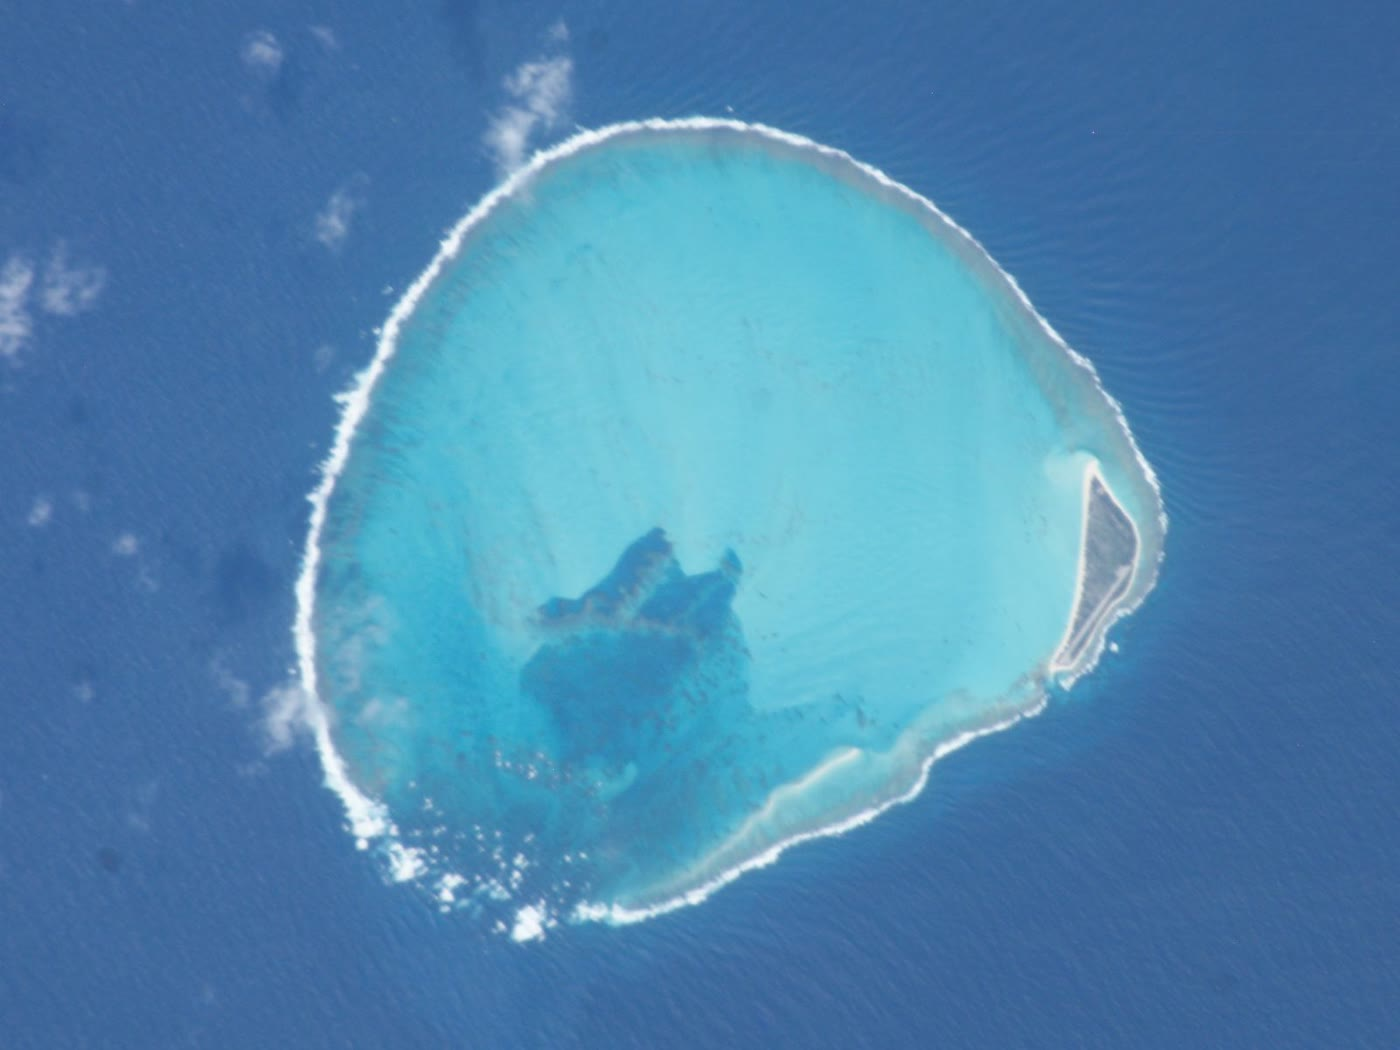
\includegraphics[width=0.52\linewidth]{images/book4/b2-17-kure-atoll.jpg}
\par\smallskip{\small L'\omterm{def:b2:oceanic-islands:reefs}{atoll} de Kure, l'\omterm{def:b2:oceanic-islands:reefs}{atoll} corallien le plus septentrional, photographié
par un astronaute depuis la Station spatiale internationale le 22 février 2004. L'anneau de
récif, large d'une dizaine de kilomètres au plus, enferme un lagon~; la seule île permanente,
Green Island, se trouve sur le bord (à droite). NASA, domaine public, via Wikimedia Commons.}
\end{omfigure}
% ledger: pmnm:kure (6 miles = 9.7 km)

\section{Érosion, niveau de la mer et fin d'une île}\label{sec:b2:oceanic-islands:erosion}

Pendant qu'elle s'enfonce, une île est aussi érodée. Une île haute capte les alizés~: sur les versants au vent
des volcans hawaïens, plus de \qty{9}{m} de pluie tombent par an en certains endroits. Les cours d'eau creusent
des canyons profonds en moins d'un million d'années, comme à Kohala, sur l'île d'Hawaï. Certaines grandes
falaises, longtemps attribuées à la seule érosion, comme les falaises marines du nord de Molokai, sont aujourd'hui
interprétées comme les niches d'arrachement de glissements géants, depuis reculées. Les vagues attaquent la côte et
aplanissent autour d'elle une plate-forme d'abrasion marine au niveau de la mer. L'érosion et l'enfoncement conjugués
font disparaître toute trace de roche volcanique au-dessus de la mer en environ \qty{15}{Ma}. Les Gardner Pinnacles,
d'à peu près le même âge, sont l'île la plus ancienne de la chaîne où de la roche volcanique se dresse encore
au-dessus de l'eau. Au-delà, vers le nord-ouest, il ne reste que des îles de sable, des \omterm{def:b2:oceanic-islands:reefs}{atolls} et des volcans noyés.
% ledger: cs14:erosion, cs14:erase

Le niveau de la mer ne reste pas immobile pendant ce temps. Au dernier maximum glaciaire, il était environ
\qty{120}{m} plus bas qu'aujourd'hui. Le littoral d'une île se trouvait alors plus bas sur ses flancs, et les récifs
qui la frangent aujourd'hui étaient des terres émergées. Lorsque la glace a fondu, la mer s'est élevée en moyenne de
\qty{12}{m} par millier d'années pendant la déglaciation principale, de 16.5 à \qty{8.2}{ka}. Pendant le Meltwater
Pulse 1A, elle s'est élevée d'au moins \qty{40}{mm} par an. Un récif posé sur un volcan qui s'enfonce doit suivre les
deux montées. Au large de la côte nord-ouest de l'île d'Hawaï, au moins six récifs noyés forment un escalier sur le
flanc, les plus anciens étant les plus profonds. Chacun a crû au rivage, a pris du retard pendant une montée de la mer,
puis a été entraîné vers le bas par la charge de la jeune île. Une fois qu'un volcan s'est enfoncé de plus d'environ
\qty{125}{m}, soit l'amplitude de la variation glaciaire du niveau de la mer, il ne remonte plus jusqu'aux vagues.
% ledger: usgs:lgm (Book 1), lambeck14:lgm (Book 2), cs14:erase, cs14:subsidence

L'arche peut agir en sens inverse. Oahu repose sur le bombement soulevé par la charge des îles plus jeunes,
et s'est un peu soulevé~: des récifs du dernier interglaciaire, âgés de 133 à \qty{115}{ka}, affleurent
tout autour de l'île, et un récif âgé d'environ \qty{334}{ka} se dresse aujourd'hui à \qty{21}{m} au-dessus
du niveau de la mer. La fin d'une \omterm{def:b2:oceanic-islands:stages}{île océanique} est donc inscrite dans ses roches et ses récifs. La lave la
bâtit, les glissements et la pluie la découpent, les vagues l'aplanissent, la plaque l'emporte vers le bas,
et un récif garde sa place à la surface jusqu'à ce que l'eau froide et une mer montante le noient à son tour.
% ledger: cs14:arch

\section*{Exercices}\label{sec:b2:oceanic-islands:exercises}

Données pour les exercices, sauf mention contraire~: loi profondeur--âge $d = \qty{2500}{m} + C\sqrt t$ avec
$C = \qty{350}{m.Ma^{-1/2}}$ pour $0 \le t \le \qty{70}{Ma}$, et $d = \qty{6400}{m} -
\qty{3200}{m}\,e^{-t/62.8}$ au-delà de \qty{20}{Ma}~; $1~\text{pied} = \qty{0.3048}{m}$, $1~\text{brasse}
= \qty{1.8288}{m}$, $1~\text{mille} = \qty{1.609}{km}$~; croissance des récifs jusqu'à \qty{4.2}{mm.an^{-1}}.

\begin{exercise}[$\star$]\label{exo:b2:oceanic-islands:1}
Nommer le stade de chaque volcan~: (a) un \omterm{def:b2:oceanic-islands:seamount}{mont sous-marin} dont le sommet est à \qty{975}{m} sous la
mer, qui émet une lave alcaline~; (b) un volcan au-dessus du point chaud, qui émet une lave tholéiitique
à fort débit~; (c) un volcan éteint dont les dernières coulées, plus alcalines que l'essentiel
de l'île, coiffent le bouclier~; (d) une île où, après un silence de \qty{2}{Ma}, quelques petits
évents alcalins s'ouvrent~; (e) un anneau de récif autour d'un lagon, sans roche volcanique en vue.
\end{exercise}

\begin{exercise}[$\star$]\label{exo:b2:oceanic-islands:2}
Un volcan est bâti sur une plaque âgée de \qty{9}{Ma}. (a) Quelle est la profondeur du fond marin qui l'entoure~?
(b) De combien se sera-t-il enfoncé lorsque la plaque aura \qty{25}{Ma}~? (c) À quel rythme s'enfonce-t-il alors~?
\end{exercise}

\begin{exercise}[$\star$]\label{exo:b2:oceanic-islands:3}
Dix-sept grands glissements se sont formés au cours des \qty{5}{Ma} passés autour des principales îles hawaïennes, et
soixante-dix le long de la dorsale hawaïenne en \qty{30}{Ma}. (a) Calculer l'intervalle moyen entre deux glissements
dans chaque cas. (b) Pourquoi ces deux intervalles ne sont-ils que des bornes supérieures de l'intervalle réel~?
\end{exercise}

\begin{exercise}[$\star$]\label{exo:b2:oceanic-islands:4}
À Enewetak, du basalte a été rencontré à 4~158 pieds dans un sondage, et le socle dur à 4~610 pieds
dans l'autre~; les coraux récifaux à la base du calcaire ne vivent pas plus profond que 150 pieds.
(a) Convertir les trois profondeurs en mètres. (b) De combien au moins le sommet du volcan sous l'île
Parry s'est-il enfoncé depuis que le premier récif s'y est développé~? (c) La base du calcaire étant
éocène, elle a au moins \qty{33.9}{Ma}. Quel est le taux moyen d'enfoncement le plus grand possible~?
\end{exercise}

\begin{exercise}[$\star\star$]\label{exo:b2:oceanic-islands:5}
(a) Calculer le taux d'enfoncement thermique, en \unit{m} par \unit{Ma} et en \unit{mm.an^{-1}},
des îles posées sur des plaques âgées de 4, 25 et \qty{49}{Ma}. (b) Combien de fois un récif
productif peut-il croître plus vite que le plus rapide de ces taux~? (c) Et combien de fois la
phase de charge au large de l'île d'Hawaï, \qty{2.6}{m} par millier d'années, est-elle plus rapide~?
\end{exercise}

\begin{exercise}[$\star\star$]\label{exo:b2:oceanic-islands:6}
(a) Avec la loi exponentielle, calculer le taux d'enfoncement sur une plaque âgée de \qty{100}{Ma}, en
\unit{m} par millier d'années, et le comparer aux \qty{0.01}{m} par millier d'années mesurés le long de
la dorsale hawaïenne. (b) Pour quel âge de plaque le taux vaut-il exactement \qty{10}{m.Ma^{-1}}~? (c)
Vérifier que les deux lois donnent presque la même profondeur pour une plaque âgée de \qty{25}{Ma}.
\end{exercise}

\begin{exercise}[$\star\star$]\label{exo:b2:oceanic-islands:7}
Les récifs hawaïens se noient environ \qty{33}{Ma} après la naissance de leur volcan, et
le volcanisme se déplace le long de la chaîne à \qty{8.6}{cm.an^{-1}}. (a) À quelle distance
du point chaud se trouve une île lorsque son récif se noie~? (b) Midway est un \omterm{def:b2:oceanic-islands:reefs}{atoll} âgé de
\qty{27.7}{Ma}~: est-il cohérent qu'il possède encore un récif vivant~? (c) Kure se trouve
à 55 milles au-delà de Midway. Estimer son âge, et dire s'il est proche du \omterm{def:b2:oceanic-islands:darwin-point}{point de Darwin}.
\end{exercise}

\begin{exercise}[$\star\star$]\label{exo:b2:oceanic-islands:8}
Dans l'\omterm{def:b2:oceanic-islands:collapse}{avalanche de débris} de Nuuanu, le \omterm{def:b2:oceanic-islands:seamount}{mont sous-marin} Tuscaloosa est un bloc long
d'environ \qty{30}{km}, large de \qty{17}{km} et haut d'au moins \qty{2}{km}. (a) Quel
volume contiendrait une boîte aux dimensions de ce bloc~? Et une pyramide de même base
et de même hauteur~? (b) Comparer avec le volume du Kilauea, \qty{10000}{km^3}. (c)
L'avalanche couvre \qty{23000}{km^2}. Si son épaisseur moyenne était de \qty{100}{m}
(une hypothèse~: son épaisseur loin d'Oahu est mal connue), quel serait son volume~?
\end{exercise}

\begin{exercise}[$\star\star$]\label{exo:b2:oceanic-islands:9}
Au large de l'île d'Hawaï, le flanc s'enfonce de \qty{2.6}{m} par millier d'années sous la charge du
volcan. (a) Combien de temps faut-il pour que le rivage s'enfonce de \qty{1}{km}~? (b) Un récif qui
croît à \qty{4.2}{mm.an^{-1}} se trouve sur ce flanc. Suit-il le rythme lorsque le niveau de la mer est
stable~? (c) Pendant la déglaciation principale, de 16.5 à \qty{8.2}{ka}, la mer s'est élevée en moyenne
de \qty{12}{mm.an^{-1}}. À quelle profondeur se trouve le sommet du récif à la fin, s'il est parti
de la surface~? (d) La même question pour un récif posé sur un volcan ancien qui ne s'enfonce plus.
\end{exercise}

\begin{exercise}[$\star\star\star$]\label{exo:b2:oceanic-islands:10}
(a) Montrer que, sur un intervalle $\Delta$ fixé, la loi en racine fait s'enfoncer une île d'autant moins que
sa plaque est ancienne. (b) Calculer l'enfoncement sur \qty{20}{Ma} pour une île née à la dorsale et pour
une île née sur une plaque âgée de \qty{50}{Ma}. (c) La plaque sous une dorsale est très chaude, et la loi en
racine donne un taux infini à $t = 0$. Est-ce un problème pour l'enfoncement sur un intervalle fini~? Expliquer.
\end{exercise}

\begin{exercise}[$\star\star\star$]\label{exo:b2:oceanic-islands:11}
Un \omterm{def:b2:oceanic-islands:reefs}{atoll} s'enfonce à \qty{30}{m.Ma^{-1}}, et le niveau de la mer oscille d'environ \qty{120}{m} avec les
âges glaciaires, par cycles d'environ \qty{100}{ka}. (a) De combien l'\omterm{def:b2:oceanic-islands:reefs}{atoll} s'enfonce-t-il pendant un
cycle~? (b) Au plus bas glaciaire, à quelle hauteur le sommet de l'\omterm{def:b2:oceanic-islands:reefs}{atoll} se dresse-t-il au-dessus de la
mer~? Que devient alors la roche récifale~? (c) Combien de cycles faut-il pour que l'\omterm{def:b2:oceanic-islands:reefs}{atoll} s'enfonce de
la totalité des \qty{120}{m}~? (d) Expliquer les zones lessivées trouvées dans les sondages d'Enewetak, et
pourquoi la \cref{prop:b2:oceanic-islands:cap} donne tout de même l'épaisseur de la coiffe à long terme.
\end{exercise}

\begin{exercise}[$\star\star\star$]\label{exo:b2:oceanic-islands:12}
Un \omterm{def:b2:oceanic-islands:reefs}{atoll} se noie lorsque sa plaque est âgée de \qty{50}{Ma}~: son récif prend du retard et son sommet s'arrête
à la limite de croissance des algues corallines les plus profondes, à \qty{150}{m} sous la mer. (a) Avec la loi
exponentielle, de combien s'enfonce-t-il encore avant que la plaque ait \qty{120}{Ma}~? (b) Quelle est la profondeur
du sommet du \omterm{def:b2:oceanic-islands:seamount}{guyot} alors~? (c) Un \omterm{def:b2:oceanic-islands:seamount}{guyot} près d'Enewetak a son sommet à 700 brasses. Convertir, et comparer. (d)
Citer deux raisons pour lesquelles un \omterm{def:b2:oceanic-islands:seamount}{guyot} réel pourrait être plus profond ou moins profond que cette estimation.
\end{exercise}

\begin{problem}[{Problème du week-end --- Du volcan à l'atoll}]\label{pb:b2:oceanic-islands:1}
L'île Petrel, imaginaire, naît au-dessus d'un point chaud sur une plaque âgée de \qty{10}{Ma}. Son volcan est
un cône de rayon à la base de \qty{50}{km}. Lorsque sa croissance prend fin, son sommet se dresse à \qty{1000}{m}
au-dessus du niveau de la mer. Sa dernière roche volcanique disparaît sous le niveau de la mer \qty{12}{Ma} plus
tard. Un récif maintient ensuite son sommet au niveau de la mer jusqu'à ce que la plaque ait \qty{70}{Ma}, moment
où l'\omterm{def:b2:oceanic-islands:reefs}{atoll} franchit le \omterm{def:b2:oceanic-islands:darwin-point}{point de Darwin}. Utiliser la loi profondeur--âge des exercices (la loi en racine jusqu'à
\qty{70}{Ma}, la loi exponentielle au-delà), une croissance récifale de \qty{4.2}{mm.an^{-1}} et les données du
chapitre. Le niveau de la mer est supposé constant, sauf dans les questions 8 à 10. Arrondir les profondeurs au mètre.

\noindent\textbf{Partie I --- Croissance.}
\begin{enumerate}
  \item Quelle est la profondeur du fond marin où naît l'île Petrel~?
  \item Quelle est la hauteur du volcan au-dessus de ce fond à la fin de sa croissance, sans tenir compte de
        l'enfoncement du fond sous la charge~?
  \item Calculer le volume du cône.
  \item Si \qty{85}{\percent} de ce volume a été émis pendant un \omterm{def:b2:oceanic-islands:stages}{stade bouclier} de \qty{1}{Ma}, quel a été le
        taux moyen d'éruption~? Comparer avec le débit actuel du Kilauea, environ
        \qty{0.1}{km^3} par an.
  \item Combien d'îles Petrel faudrait-il pour égaler un Mauna Loa, de \qty{95600}{km^3}~?
  \item Quelles laves, tholéiitiques ou alcalines, forment l'essentiel du cône~? Lesquelles le coiffent~?
\end{enumerate}

\noindent\textbf{Partie II --- Charge et récifs noyés.}
\begin{enumerate}[resume]
  \item Pendant sa croissance, la charge fait s'enfoncer la jeune île de \qty{1}{km} en \qty{1}{Ma}. Quel est le
        taux moyen, et comment se compare-t-il aux \qty{2.6}{m} par millier d'années mesurés
        au large de l'île d'Hawaï~?
  \item Un récif croît sur le rivage pendant cette phase, le niveau de la mer restant stable. Suit-il le rythme, et
        avec quelle marge~?
  \item Le niveau de la mer monte ensuite de \qty{12}{mm.an^{-1}}. De combien le récif prend-il du retard chaque
        année~?
  \item Au bout de combien de temps son sommet atteint-il \qty{150}{m}, la limite de croissance la plus profonde~? Que cela
        laisse-t-il sur le flanc de l'île~?
\end{enumerate}

\noindent\textbf{Partie III --- Enfoncement et érosion.}
\begin{enumerate}[resume]
  \item De combien l'île Petrel s'est-elle enfoncée au moment où sa dernière roche volcanique disparaît, la
        plaque ayant alors \qty{22}{Ma}~?
  \item Quelle part des \qty{1000}{m} du sommet a été enlevée par l'érosion, et à quel taux moyen~?
  \item À quel rythme l'île Petrel s'enfonce-t-elle à la fin de sa croissance, puis au moment où son sommet disparaît~?
  \item À quelle profondeur se trouve alors le fond marin qui l'entoure~?
  \item Comparer les \qty{12}{Ma} qu'il lui a fallu aux \qty{15}{Ma} des îles Hawaï. Donner une
        raison pour laquelle une haute île hawaïenne dure plus longtemps.
  \item Citer deux processus, outre la pluie et les rivières, qui retirent l'île au-dessus du niveau de la mer.
  \item Quelle forme de récif entoure l'île Petrel peu avant la disparition de son sommet~?
\end{enumerate}

\noindent\textbf{Partie IV --- Atoll et guyot.}
\begin{enumerate}[resume]
  \item Quelle est l'épaisseur de la coiffe récifale lorsque la plaque est âgée de \qty{70}{Ma}~?
  \item Quel taux moyen de croissance récifale cela suppose-t-il~? Combien de fois est-il inférieur à la croissance
        que le récif pourrait atteindre~?
  \item Comparer la coiffe à la profondeur du basalte sous Enewetak.
  \item À quelle profondeur se trouve le fond marin autour de l'\omterm{def:b2:oceanic-islands:reefs}{atoll} lorsqu'il franchit le \omterm{def:b2:oceanic-islands:darwin-point}{point de Darwin}~?
  \item Avec la loi exponentielle, de combien l'\omterm{def:b2:oceanic-islands:reefs}{atoll} noyé s'enfonce-t-il encore avant que la plaque ne soit
        âgée de \qty{120}{Ma}~?
  \item Si le sommet du récif s'est arrêté à \qty{150}{m} au moment de sa noyade, à quelle profondeur se trouve le sommet du
        \omterm{def:b2:oceanic-islands:seamount}{guyot} à cet instant~?
  \item En résumé~: quelle est l'épaisseur de la coiffe récifale de l'\omterm{def:b2:oceanic-islands:reefs}{atoll} Petrel~?
\end{enumerate}
\end{problem}
